\chapter{Coupling an existing MODFLOW 6 model}\label{ch:existing}

\begin{plain}
You give Raven your MODFLOW~6 model and tell it three things: where the model lies on the map, on what calendar date the
model's time starts, and which of the model's packages Raven should replace --- usually recharge and evaporation, which Raven
now supplies. Raven copies the model, makes the few changes shown in Figure~\ref{fig:workcopy}, and runs the copy together
with the Raven model, one day at a time. Your own files are never changed.
\end{plain}

Many users already have a calibrated MODFLOW~6 model and want to connect it to a Raven model. In this mode Raven does not
build a groundwater model. It takes the user's model as it is: the grid, the layers, the conductivities, storage, wells,
boundaries, stress periods and solver settings. Raven links its HRUs to the model's top active layer --- the highest layer
that holds water at each location --- and exchanges water there.

Only three things change, and only in a copy of the model (Figure~\ref{fig:workcopy}):
\begin{enumerate}
\item the stress periods are split into Raven time steps;
\item the packages that Raven takes over (usually recharge and evapotranspiration) are switched off;
\item two packages are added: \cmd{RCH\_RAVEN} (recharge from Raven) and \cmd{DRN\_RAVEN} (seepage back to Raven).
\end{enumerate}

\begin{figure}[!htbp]\centering% The working copy of an existing model (TikZ)
\begin{tikzpicture}[every node/.append style={execute at begin node={\hyphenpenalty=10000\exhyphenpenalty=10000}},font=\sffamily\small,arr/.style={-{Stealth[length=2.4mm]},line width=0.9pt}]
\node[draw=black!55,rounded corners=3pt,line width=0.8pt,fill=white,inner sep=6pt,align=left,anchor=north west] (L) at (0,0) {%
  \textbf{Your model folder}\\[1pt]{\itshape\color{teal!70!black}never changed}\\[5pt]
  {\footnotesize\ttfamily\begin{tabular}{l}mfsim.nam\\.tdis\\.dis .npf .sto .ic\\.wel .riv .ghb\\.rcha .evta\\.ims .oc\end{tabular}}};
\node[draw=brand,rounded corners=3pt,line width=0.8pt,fill=brandlight,inner sep=6pt,align=left,anchor=north west] (R) at ([xshift=16mm]L.north east) {%
  \textbf{Working copy in \texttt{output/mf6/}}\\[5pt]
  {\footnotesize\begin{tabular}{l@{\hspace{3mm}}l}
  \texttt{mfsim.nam} & unchanged\\
  \textcolor{orange!80!black}{\texttt{.tdis}} & \textcolor{orange!80!black}{periods split into Raven's days}\\
  \texttt{.dis .npf .sto .ic} & unchanged\\
  \texttt{.wel .riv .ghb} & kept; rivers exchange with Raven\\
  \textcolor{red!65!black}{\texttt{.rcha .evta}} & \textcolor{red!65!black}{switched off: Raven takes over}\\
  \textcolor{teal!70!black}{\texttt{+ raven.rch}} & \textcolor{teal!70!black}{added: recharge from Raven daily}\\
  \textcolor{teal!70!black}{\texttt{+ raven.drn}} & \textcolor{teal!70!black}{added: seepage to Raven daily}\\
  \end{tabular}}};
\draw[arr,brand] (L.east |- R.center) -- node[above,font=\sffamily\bfseries\footnotesize,text=brand]{copied} (R.west |- R.center);
\node[draw=teal!70!black,rounded corners=3pt,line width=0.8pt,fill=teal!7,inner sep=6pt,anchor=north] (B) at ([yshift=-8mm]current bounding box.south) {Raven runs this copy through MODFLOW's library, one day at a time.};
\draw[arr,teal!70!black] (R.south) -- (R.south |- B.north);
\end{tikzpicture}

\caption{Raven runs a working copy of the model. The copy differs from the original in three ways only; the original folder is never changed.}\label{fig:workcopy}
\end{figure}

The approach follows L.~Scantlebury's MODFLOW-USG coupling, which linked the top layer of an existing model to HRUs
through a table of overlap weights. It works for any grid, because only the top layer is linked and the model's cells are
found through MODFLOW's own memory. Regular (DIS) and polygon (DISV) grids are supported.

\section{A complete example}
\begin{lstlisting}
# Liard.rvg - Raven coupled to an existing MODFLOW 6 model
:HRUGeometry      Liard_HRUs.geojson  HRU_ID       # HRU polygons (lon/lat)
:MF6Library       /opt/mf6/libmf6.so
:MF6Simulation    model/mfsim.nam                  # the existing simulation
:MF6CRS           EPSG:32610                       # projection of the model's coordinates
:MF6StartDate     1985-10-01                       # date of the model's time zero
:RavenTakesOver   RCH_MODEL EVT_MODEL              # packages Raven replaces
:StreamPackage    RIV_STREAMS AUX SUBBASIN         # river cells linked to Raven's reaches
:SeepageToRaven   ON                               # groundwater seeping out returns to Raven
\end{lstlisting}
HRUs with an \cmd{AQUIFER\_PROFILE} in the \cmd{.rvh} file are coupled, as in the generated mode; with an existing model
the profile's layers are not used, only its seepage parameters (\cmd{SEEPAGE\_LEAKANCE}, \cmd{SEEPAGE\_SMOOTHING\_DEPTH}).
Raven's recharge must reach the \cmd{GROUNDWATER} store, exactly as in Section~\ref{sec:buildparams}.

\section{Linking HRUs to the model's cells}
Raven needs to know which grid cells lie under each HRU. MODFLOW model files do not say where on Earth the model is, so the
user supplies that information in one of three ways (give exactly one). Each coupled HRU is then linked to the top active
cell of every column it overlaps.

\paragraph{\cmd{:MF6CRS} (recommended).} The user names the model's map projection, usually as a standard EPSG code. Raven
reads the cell outlines from the model itself (column and row widths, origin and rotation for DIS grids; the cell corners for
DISV grids) and places them on the map with that projection (Figure~\ref{fig:placing}).
\begin{figure}[!htbp]\centering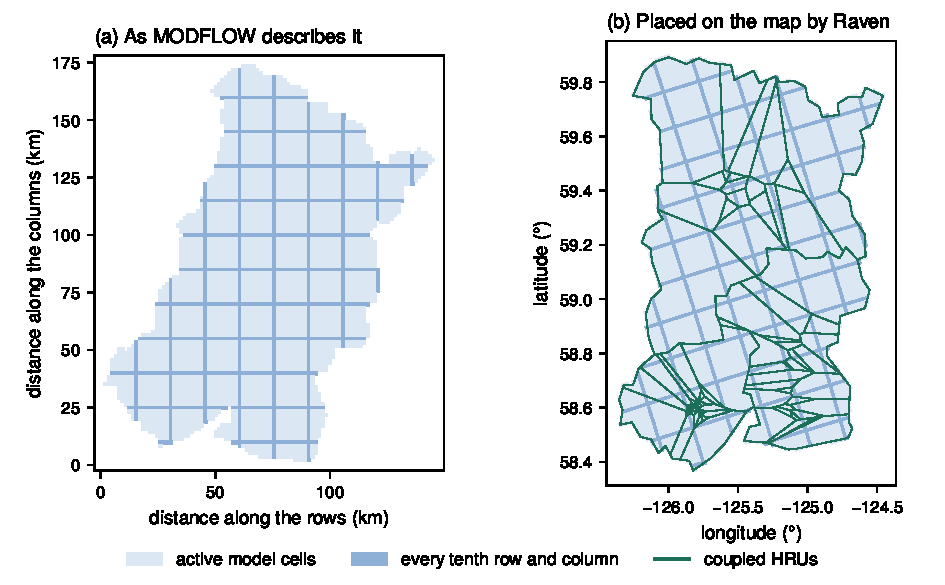
\includegraphics[width=0.95\linewidth]{figures/fig_placing.pdf}
\caption{The synthetic Liard model's cells: (a) as MODFLOW describes them, in the model's own rotated coordinates; (b) placed on the map by Raven from the projection \cmd{EPSG:32610}, under the Raven HRUs.}\label{fig:placing}
\end{figure}
 Built-in projections need no external software: Transverse Mercator (every UTM zone, north and south), Albers
equal-area and Lambert conformal conic, on the WGS84 or GRS80 (NAD83) ellipsoid. Common codes are recognised directly:
\begin{center}\small
\begin{tabularx}{\linewidth}{P{0.46\linewidth}Y}\toprule\hdr
Code & Projection\\\midrule
\cmd{EPSG:32601}--\cmd{32660}, \cmd{EPSG:32701}--\cmd{32760} & WGS84 / UTM zones, north and south\\
\cmd{EPSG:26901}--\cmd{26923} & NAD83 / UTM zones 1--23 north\\
\cmd{EPSG:3005} & NAD83 / BC Albers\\
\cmd{ESRI:102001} (or \cmd{EPSG:102001}) & Canada Albers equal-area conic (an ESRI code)\\
\cmd{EPSG:5070} & NAD83 / CONUS Albers\\
\cmd{EPSG:3978}, \cmd{EPSG:3347} & NAD83 / Canada Atlas Lambert; Statistics Canada Lambert\\\bottomrule
\end{tabularx}\end{center}
Any other projection of these three kinds is given by its parameters:
\begin{lstlisting}
:MF6CRS TMERC  lat0 lon0 k0 FE FN {WGS84|GRS80}
:MF6CRS ALBERS lat1 lat2 lat0 lon0 FE FN {WGS84|GRS80}
:MF6CRS LCC    lat1 lat2 lat0 lon0 FE FN {WGS84|GRS80}
\end{lstlisting}
The built-in formulas (Karney's series for Transverse Mercator, Snyder's for the conics) agree with the PROJ library to a few
micrometres (Section~\ref{sec:vexisting}). The small datum difference between NAD83 and WGS84 (about a metre) is ignored.

\paragraph{\cmd{:MF6GridFile}.} A GeoJSON file of the top-layer cells in longitude/latitude, numbered by an ID field
(default \cmd{CELL\_ID}) from 1 to the number of cells in a layer, as exported by GIS software. Raven checks that there is one
polygon per cell and that the polygons are the model's cells in the model's order. A map projection scales areas and turns
directions slightly, so Raven allows one common scale and one common rotation, and nothing else:
\begin{itemize}
\item every polygon's area, divided by the area MODFLOW gives the cell, must be the same for all cells within 5\%, and this
      common ratio must lie between 0.8 and 1.25 (a wrong length unit gives about 0.09 or 10.8);
\item for every pair of neighbouring cells MODFLOW connects, the two polygons must lie as far apart and in the same direction
      as MODFLOW's cells, within 20\% and 15\textdegree{} after the common scale and rotation. A shuffled numbering changes
      the distances; a mirrored one (for example rows numbered from the south: MODFLOW's row 1 is the northern row) turns
      directions around.
\end{itemize}
A file that fails either check stops the run with a message naming the first cell that does not fit.
\cmd{GWModelSummary.txt} reports the common area ratio.

\paragraph{\cmd{:OverlapWeights}.} The table of the MODFLOW-USG coupling, prepared outside Raven:
\begin{lstlisting}
:OverlapWeights
  # [HRU ID] [cell] [w = overlap area / cell area]
  2736   1204   0.35
  2736   1205   1.0
:EndOverlapWeights
\end{lstlisting}
No HRU polygons are needed. Monitoring wells cannot be located with this option.

\paragraph{No water is lost on the way.} Each HRU's recharge is shared among the cells it covers, in proportion to how much of
the HRU lies in each cell (Figure~\ref{fig:linking}a). The shares always add up to 100\%, so all the water Raven sends
arrives in MODFLOW --- even when the HRU polygons or the weights do not quite match the HRU areas in the \cmd{.rvh} file. A
mismatch changes only \emph{where} inside the HRU the water lands, not \emph{how much} (Figure~\ref{fig:linking}b). In
formula form, cell $i$ receives $V_{k\to i}=R_k\,A_k\,A_{ki}/\sum_j A_{kj}$ from HRU $k$ (Section~\ref{sec:linkage}).

\begin{figure}[!htbp]\centering% HRU over grid cells with its share in each cell (generated by make_tikz_linking.py; shares computed from the shapes)
\begin{tikzpicture}[x=1mm,y=1mm,font=\sffamily\footnotesize,every node/.append style={execute at begin node={\hyphenpenalty=10000\exhyphenpenalty=10000}}]
\node[anchor=south west,font=\sffamily\small] at (0,43) {(a) The HRU's share in each cell};
\fill[teal!18] (5.46,4.94) -- (19.50,3.64) -- (32.50,6.50) -- (46.80,4.29) -- (45.50,19.50) -- (47.58,34.06) -- (31.20,35.62) -- (19.50,32.76) -- (4.42,35.10) -- (6.76,19.50) -- cycle;
\draw[black!45,line width=0.4pt] (0,0) rectangle (13,13);
\draw[black!45,line width=0.4pt] (0,13) rectangle (13,26);
\draw[black!45,line width=0.4pt] (0,26) rectangle (13,39);
\draw[black!45,line width=0.4pt] (13,0) rectangle (26,13);
\draw[black!45,line width=0.4pt] (13,13) rectangle (26,26);
\draw[black!45,line width=0.4pt] (13,26) rectangle (26,39);
\draw[black!45,line width=0.4pt] (26,0) rectangle (39,13);
\draw[black!45,line width=0.4pt] (26,13) rectangle (39,26);
\draw[black!45,line width=0.4pt] (26,26) rectangle (39,39);
\draw[black!45,line width=0.4pt] (39,0) rectangle (52,13);
\draw[black!45,line width=0.4pt] (39,13) rectangle (52,26);
\draw[black!45,line width=0.4pt] (39,26) rectangle (52,39);
\draw[teal!70!black,line width=1.1pt] (5.46,4.94) -- (19.50,3.64) -- (32.50,6.50) -- (46.80,4.29) -- (45.50,19.50) -- (47.58,34.06) -- (31.20,35.62) -- (19.50,32.76) -- (4.42,35.10) -- (6.76,19.50) -- cycle;
\node[font=\sffamily\bfseries\scriptsize,text=teal!45!black,inner sep=0.5pt] at (9.37,8.21) {5\%};
\node[font=\sffamily\bfseries\scriptsize,text=teal!45!black,inner sep=0.5pt] at (9.67,22.57) {7\%};
\node[font=\sffamily\bfseries\scriptsize,text=teal!45!black,inner sep=0.5pt] at (9.10,30.37) {6\%};
\node[font=\sffamily\bfseries\scriptsize,text=teal!45!black,inner sep=0.5pt] at (19.17,8.35) {10\%};
\node[font=\sffamily\bfseries\scriptsize,text=teal!45!black,inner sep=0.5pt] at (19.50,19.50) {14\%};
\node[font=\sffamily\bfseries\scriptsize,text=teal!45!black,inner sep=0.5pt] at (22.24,29.67) {8\%};
\node[font=\sffamily\bfseries\scriptsize,text=teal!45!black,inner sep=0.5pt] at (29.53,9.47) {8\%};
\node[font=\sffamily\bfseries\scriptsize,text=teal!45!black,inner sep=0.5pt] at (32.50,19.50) {14\%};
\node[font=\sffamily\bfseries\scriptsize,text=teal!45!black,inner sep=0.5pt] at (31.56,30.78) {10\%};
\node[font=\sffamily\bfseries\scriptsize,text=teal!45!black,inner sep=0.5pt] at (42.70,8.71) {5\%};
\node[font=\sffamily\bfseries\scriptsize,text=teal!45!black,inner sep=0.5pt] at (42.43,22.47) {7\%};
\node[font=\sffamily\bfseries\scriptsize,text=teal!45!black,inner sep=0.5pt] at (43.05,30.47) {6\%};
\node[anchor=north,align=center,text width=50mm] at (26,-2) {One HRU (green) over 12 grid cells.\\The shares add up to 100\%.};
\node[anchor=south west,font=\sffamily\small] at (64,43) {(b) 10\,mm of recharge on a 5\,km$^2$ HRU};
\node[anchor=south west,align=left,inner sep=0pt] at (64,36.2) {Raven sends};
\fill[brand] (64,30.5) rectangle (112,35.5);
\node[anchor=west] at (113.5,33) {50\,000\,m$^3$};
\node[anchor=south west,align=left,inner sep=0pt] at (64,22.2) {Arrives if the weights are used as they are\\(here they add up to only 92\%)};
\fill[red!65!black] (64,16.5) rectangle (108.16,21.5);
\draw[red!65!black,pattern=north east lines,pattern color=red!65!black] (108.16,16.5) rectangle (112,21.5);
\node[anchor=west,text=red!65!black] at (113.5,19) {46\,000\,m$^3$ \ (4\,000\,m$^3$ lost)};
\node[anchor=south west,align=left,inner sep=0pt] at (64,8.2) {Arrives with Raven's shares, which always\\add up to 100\%};
\fill[teal!70!black] (64,2.5) rectangle (112,7.5);
\node[anchor=west] at (113.5,5) {50\,000\,m$^3$};
\end{tikzpicture}

\caption{Sharing an HRU's water among cells. (a) The HRU's share in each cell, computed from the shapes; the shares add up to 100\%. (b) Weights that add up to only 92\% would lose 8\% of the water; Raven's shares always add up to 100\%, so every cubic metre arrives.}\label{fig:linking}
\end{figure}

In the older MODFLOW-USG coupling the weights were used as given, so the recharge volume depended on how carefully the HRUs
were drawn. Rates passed to MODFLOW use MODFLOW's own cell areas. \cmd{GWModelSummary.txt} reports how much of the coupled
HRUs' area lies on active cells; a low value usually means a wrong projection or HRUs outside the model.

\section{Time}\label{sec:existingtime}
MODFLOW models divide time into \emph{stress periods}: stretches of time, often a month, during which inputs such as pumping
rates stay the same. Raven works in days. Raven keeps the model's stress periods and their dates, and splits each period into
Raven days (Figure~\ref{fig:periods}), so the model's own changes --- a well pumping harder in summer, a boundary level
changing --- still happen on their dates.

\cmd{:MF6StartDate} is the calendar date on which the model's time starts. Each stress period must contain a whole number of
Raven time steps, and Raven's run may not go past the end of the model; otherwise the run stops with a message. Steady-state
periods (solved as the long-term balance) stay steady-state.

\paragraph{Steady-state models.} Many calibrated models are steady state: no storage package (or one that marks every period
steady) and a single stress period whose length has no meaning (often one second or one day). Raven stretches that period
over its run, so every Raven step is a steady-state solution with that step's recharge: the aquifer responds at once, without
storage. \cmd{GWModelSummary.txt} says so, and the storage column of \cmd{GWBudget.csv} stays zero (the balance residual is
reported as MODFLOW's error). Because such a model has no time of its own, Raven may start on any date from
\cmd{:MF6StartDate} on.

\begin{figure}[!htbp]\centering% Stress periods, Raven's days and a restart after 40 days (TikZ; 1 mm per day)
\begin{tikzpicture}[every node/.append style={execute at begin node={\hyphenpenalty=10000\exhyphenpenalty=10000}},x=1mm,y=1mm,font=\sffamily\footnotesize,
  rowlab/.style={anchor=east,align=right,text width=25mm,font=\sffamily\footnotesize\bfseries},
  per/.style={draw=brand,fill=brandlight,line width=0.6pt},
  new/.style={draw=teal!70!black,fill=teal!8,line width=0.6pt}]
% row 1: the model's stress periods (1 steady day, then 31, 30, 31, 31 days)
\node[rowlab,text=brand] at (-3,0) {Model's stress\\periods};
\draw[per] (0,-4) rectangle (1,4);
\foreach \a/\b/\t/\lx in {1/32/{2 \ (31 days)}/16.5, 32/62/{3 \ (30 days)}/52, 62/93/{4 \ (31 days)}/77.5, 93/124/{5 \ (31 days)}/108.5}{
  \draw[per] (\a,-4) rectangle (\b,4); \node at (\lx,0) {\t};}
\draw[black!60] (0.5,4) -- (0.5,8.5) node[above,align=center,font=\sffamily\scriptsize] {1: steady\\(1 day)};
% row 2: Raven's days
\node[rowlab,text=black!70] at (-3,-11) {Raven's days};
\foreach \d in {0,...,124}{\draw[black!45,line width=0.3pt] (\d,-12.5) -- (\d,-9.5);}
% row 3: after a restart after 40 days
\node[rowlab,text=teal!70!black] at (-3,-24) {After a restart\\after 40 days};
\draw[black!45,fill=black!6,pattern=north east lines,pattern color=black!30] (0,-28) rectangle (40,-20);
\node[fill=white,inner sep=1.5pt,text=black!65] at (20,-24) {already simulated: dropped};
\foreach \a/\b/\t in {40/62/{1 \ (22 days)}, 62/93/{2 \ (31 days)}, 93/124/{3 \ (31 days)}}{
  \draw[new] (\a,-28) rectangle (\b,-20); \node at ({(\a+\b)/2},-24) {\t};}
% the restart
\draw[red!65!black,dashed,line width=0.9pt] (40,12) -- (40,-30);
\node[above,text=red!65!black,font=\sffamily\bfseries\footnotesize] at (40,12) {restart};
\end{tikzpicture}

\caption{Top: a model with a one-day steady period followed by periods of 31, 30, 31 and 31 days, and Raven's days. Bottom: after a restart 40 days into the model, the time already simulated is dropped, period~3 keeps its last 22 days, and the periods are renumbered; each keeps its own well rates and boundary levels.}\label{fig:periods}
\end{figure}

\paragraph{Starting later: restarts.} Raven may start later than the model's time zero --- when a run is continued from
\cmd{solution.rvc}, or begins part-way through the model. Raven then removes the stress periods already simulated from the
working copy, shortens the period that holds Raven's start, and renumbers the periods of every package; the new first period
takes the inputs that were in force on Raven's start date (Figure~\ref{fig:periods}, bottom). This is safe for packages whose period
entries replace one another (WEL, RIV, GHB, CHD, DRN, list-based RCH and EVT, STO, OC, the water mover MVR), and for
array-based recharge and ET and the advanced packages (SFR, LAK, MAW, UZF) when at most one period entry comes before Raven's
start. Such a package with several earlier entries, whose settings build on one another, stops such a run, as do time-varying conductivity or storage
(\cmd{TVK6}, \cmd{TVS6}) and a simulation holding more than one model (only the coupled model's periods would be
renumbered); Raven must then start at \cmd{:MF6StartDate}. A package that uses time series stops any later start, even one
inside the first period, because the times of a series count from the model's own start. A time of day in Raven's
\cmd{:StartDate} counts in the offset, and the working copy's \cmd{START\_DATE\_TIME} is set to Raven's start.

\section{Units}
Length units (metres, feet, centimetres) are read from the discretization package and time units (seconds to years) from
the time discretization. Heads, flows, rates, conductances and coordinates are converted at the interface; Raven's outputs
are always in metres and days.

\section{Packages}
\begin{table}[!htbp]\centering
\caption{How the model's packages are treated.}\label{tab:extpkgs}
\begin{tabularx}{\linewidth}{P{0.30\linewidth}Y}\toprule\hdr
Package & Treatment\\\midrule
Recharge, evapotranspiration, UZF & must be named in \cmd{:RavenTakesOver} (removed; Raven supplies recharge) or in \cmd{:KeepPackages} (they stay). An undeclared one stops the run, so recharge is never counted twice\\
Stream package (\cmd{:StreamPackage}) & a RIV, DRN or GHB package whose flows go to Raven's reaches: to the subbasin in an auxiliary variable (\cmd{AUX} name, default \cmd{SUBBASIN}), or to the subbasin of the dominant HRU of the cell (\cmd{DOMINANT\_HRU}). Losing reaches take the water from the channel; a loss that cannot be supplied is carried to the next step\\
\cmd{DRN\_RAVEN} (\cmd{:SeepageToRaven ON}) & added at the top of the top active cell of coupled columns; the discharge returns to Raven (Section~\ref{ch:seepage})\\
\cmd{RCH\_RAVEN} & added at the top active cell of every coupled column. MODFLOW ignores recharge on specified-head cells, so columns whose top cell is specified-head (read from the model each step, as the stress periods may change them) take none: each HRU's recharge is spread over its other cells, and recharge of an HRU lying only on such cells is reported in \cmd{GWBudget.csv} (\emph{recharge onto CHD cells})\\
Water mover (MVR) & kept; movers from or to a package Raven takes over are removed from the working copy (MODFLOW would stop on a package that is no longer there), and \cmd{GWModelSummary.txt} reports how many. A stream package that sends water through the mover is refused, because Raven would take the same water from the aquifer a second time\\
All other packages & kept unchanged: wells, head boundaries, drains, lakes, streamflow routing and so on. Their simulated flows, including the water they pass to the mover, enter the balance check (\cmd{GWBudget.csv}, column \emph{other model packages})\\\bottomrule
\end{tabularx}
\end{table}

\section{Safeguards}
Every one of these stops the run with a message that names the problem and the fix:
\begin{itemize}
\item a recharge, ET or UZF package not declared taken over or kept; \cmd{:RavenTakesOver} naming another kind of package;
      a stream package that is not RIV, DRN or GHB, or one that sends water through the mover; a package name not in the
      model name file; a mover whose period data sit in another file, when it names a package Raven takes over;
\item several groundwater models in the simulation and no \cmd{:MF6Model};
\item a Raven start before the model's time zero (\cmd{:MF6StartDate}); a later start that the model's packages cannot follow (Section~\ref{sec:existingtime}); a stress period that is not a whole number of Raven steps; a Raven run longer than
      the model;
\item a cell file whose polygons are not the model's cells (count, numbering or area);
\item a stream cell whose subbasin does not exist or is disabled;
\item options of the generated mode left in the \cmd{.rvg} file (grid options, \cmd{:GridCellSize}, \cmd{:LandSurface},
      \cmd{:BedrockSurface}, the solver settings, \cmd{:Wells}, head boundaries, \cmd{:RiverGeometry}, \cmd{:GWInitialization}),
      or none or several ways of linking HRUs;
\item a simulation with more than one solution (for example a transport model with its own IMS): Raven drives one
      groundwater-flow solution;
\item adaptive time stepping (\cmd{ATS6} in the TDIS options): Raven needs fixed time steps;
\item a Raven calendar other than Gregorian (the dates of the two models are compared day by day);
\item \cmd{:WriteNetCDFHeads} with \cmd{:OverlapWeights} (a weight table has no coordinates);
\item a simulation that lies inside Raven's own working folder (\cmd{output/mf6/}), which Raven overwrites.
\end{itemize}
A solver tolerance looser than 0.01 m is reported in \cmd{GWModelSummary.txt}.

\section{The model's solver}
The model's own solver settings (\cmd{.ims}) are used. On a step that needs more than 100 outer iterations (or half the
model's iteration limit, if that is smaller) the coupler relaxes
MODFLOW's head tolerance tenfold for the rest of that step (as for generated models, Section~\ref{ch:mf6}), in the model's
units. The first coupled step is often the hardest --- a steady-state period solved from the model's starting heads with
Raven's recharge --- so allow at least 500 outer iterations (\cmd{OUTER\_MAXIMUM}). A step that does not converge is flagged
in \cmd{GWBudget.csv} and the exchange on it is limited, as described in Section~\ref{ch:mf6}. For this, the working copy's
\cmd{mfsim.nam} always has the \cmd{CONTINUE} option: without it, MODFLOW would stop the whole simulation at the first step
that does not converge.

With MODFLOW versions before 6.8, the \cmd{UNDER\_RELAXATION} keyword of the model's \cmd{NEWTON} option can make a step in
which a cell dries repeat the same Newton change at every iteration and never converge (the synthetic Liard model failed on
every day with MODFLOW~6.6.3 and converged on every day with 6.8.1). Raven reads the library's version, writes it
to \cmd{GWModelSummary.txt}, and warns when an older version meets that keyword: use MODFLOW~6.8 or newer, or remove the
keyword from the model's name file (on the synthetic model the results with 6.8.1 are identical either way).

\section{Outputs and restarts}
All outputs of Chapter~\ref{ch:c6} are written. Raven copies the whole folder that holds the simulation file (the simulation
may read files from anywhere in it), so keep the model in a folder of its own; old results (\cmd{.hds}, \cmd{.cbc},
\cmd{.lst}, \cmd{.grb}, \cmd{.bud}, \cmd{.cbb}) are not copied. The simulation file may have any name: the working copy
always holds it as \cmd{mfsim.nam}, the name MODFLOW's library opens. In \cmd{GWHRUState.csv} the water-table depth is
measured from the top of the model's top active cell, which with an existing model stands for the land surface. \cmd{mf6/} holds the working copy of the simulation, with Raven's packages
(\cmd{raven.rch}, \cmd{raven.drn}); \cmd{mf6/grid\_cells.geojson} shows the linked cells (not with \cmd{:OverlapWeights}).
Restarts store the heads in the model's layout (\cmd{:GWHeads} \emph{nlay nrow ncol} for DIS, \emph{nlay} \cmd{1} \emph{ncells}
for DISV); on a restart Raven writes them as the initial heads of the working copy (\cmd{raven.ic}) and renumbers the stress
periods as described above. A restarted run reproduces a continuous one (Section~\ref{sec:vexisting}).

\section{Worked example}
\cmd{examples/Liard\_existing\_model/} holds a MODFLOW 6 model of the Liard coupled area built independently of Raven: a
regular grid of 1.5 km cells rotated 15\textdegree{} in UTM zone 10N, four layers with spatially varying conductivity,
a one-day steady-state period followed by 24 monthly periods, two wells with seasonal pumping, 239 river cells carrying
their subbasin ID in an auxiliary variable, a head boundary at the outlet, and its own recharge and ET packages. The \cmd{.rvg}
file of Section~\ref{ch:existing} couples it to the Liard Raven model; the two-year run takes about four minutes.

\section{Checking the calibration}
Replacing a calibrated recharge package with Raven's recharge changes the model's water budget. Compare the coupled heads and
budget with a run of the original model before using the results: large differences mean Raven's recharge, or the
recharge the model was calibrated with, needs attention.

\section{Current limits}
DISU models, water-table ET from Raven (the model's own ET package can be kept), surface-store and reservoir exchanges, and
the conductance limit of generated river cells are not available in this mode; the stream package's stage comes from the
model. Restarts after the model's time zero need daily or longer Raven time steps.
